\chapter{Site Web}

\section{Objectifs}

Le site web fut principalement un moyen de présenter, de façon graphique, le résultat des différentes parties abordées durant ce projet. Pour la première partie, il consistait à afficher, grâce à l'utilisation des diagrammes, les statistiques de notre étude sur les certificats. Pour la deuxième partie, nous avons souhaité présenter le rapport d'audit au format HTML, celui-ci a également été livré lors de la deuxième livraison au format LaTeX. Enfin, notre site fut aussi une plate-forme pour l'intégration de la troisième partie du projet qui consiste à tester le navigateur du client. \\


\section{Statistiques}

Après quelques recherches, nous nous sommes mis d'accord sur l'utilisation de l'application \textit{javascript} \textit{Highcharts} pour la représentation des différents diagrammes sur le site. L'utilisation est simple et variée, nous l'avons utilisé de trois façons différentes : 
\begin{itemize}
\item \textbf{Statique} : données sont récupérées directement depuis un tableau HTML ;
\item \textbf{Dynamique} : données sont récupérées depuis la base de données ;
\item \textbf{AJAX} : données sont récupérées par des appels AJAX.\\
\end{itemize}

Chaque diagramme possède une fonctionnalité \textit{tooltip} qui offre plus d'informations sur les données représentées. Il est actionné lors du passage de la souris sur une part du cadre du diagramme circulaire (cf. figure \ref{taille_clefs})

\subsection{Statistiques Générales}

Nous avons souhaité faire une comparaison entre les deux scans réalisés durant le développement de la première partie du projet. De ce fait, nous présentons sur un même diagramme la proportion des certificats récupérés et ceux qui sont vulnérables pour le premier et deuxième scan. On y affiche également un tableau contenant, en chiffres, les valeurs du diagramme ainsi que le pourcentage de certificats vulnérables sur l'ensemble récupéré.

\begin{figure}[H]
\begin{center}
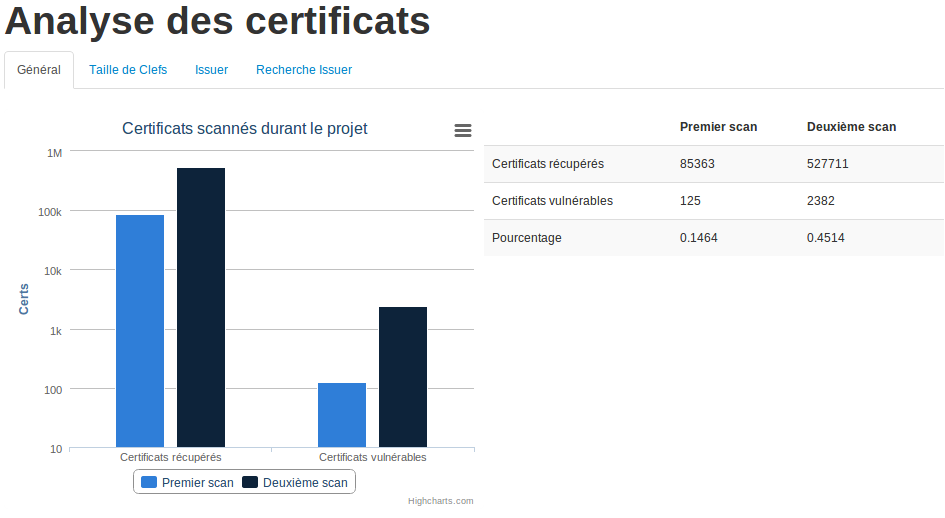
\includegraphics[scale=0.5]{images/site_web_stats_gen.png}
\end{center}
\caption{Site Web - Statistique Général}
\label{stats_general}
\end{figure}

\subsection{Taille des clefs}

On représente ici, avec un diagramme circulaire, les tailles des clefs des certificats récupérés. De tout les certificats se trouvant sur notre base de données, on identifie ceux possédant une taille de clef allant de 512 octets à 16.384 octets.

\begin{figure}[H]
\begin{center}
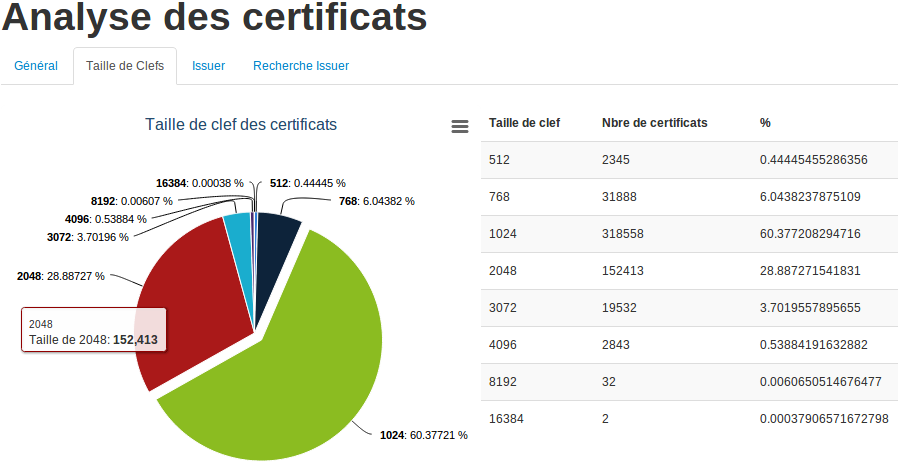
\includegraphics[scale=0.5]{images/site_web_stats_clefs.png}
\end{center}
\caption{Site Web - Taille de clef}
\label{taille_clefs}
\end{figure}

\subsection{Les émetteurs}

Cette partie représente un tableau de tous les émetteurs se trouvant sur notre base de données. On y récupère aussi, à l'aide de deux requêtes SQL, le nombre total de certificats que possède chacun des émetteur ainsi que le nombre de certificats vulnérables.

\begin{figure}[H]
\begin{center}
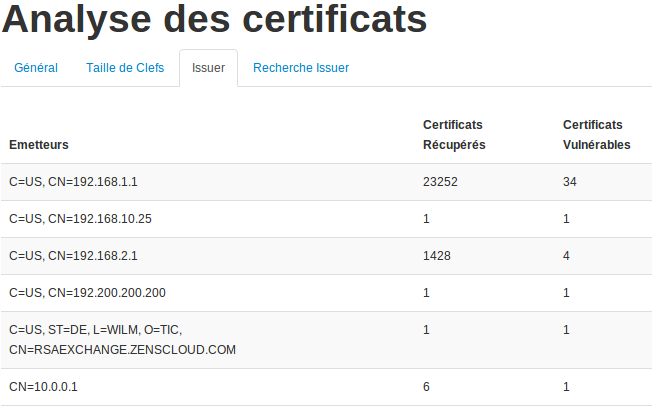
\includegraphics[scale=0.5]{images/site_web_issuer.png}
\end{center}
\caption{Site Web - Emetteurs}
\label{issuer}
\end{figure}

\subsection{Onglet de recherche}

Nous avons également intégré une barre de recherche. L'utilisateur peut ainsi faire une recherche avancée, en choisissant parmi les critères suivants :
\begin{itemize}
\item Le sujet (\textit{subject} ;
\item L'émetteur (\textit{issuer}) ;
\item La taille de la clef.\\
\end{itemize}

\begin{figure}[H]
\begin{center}
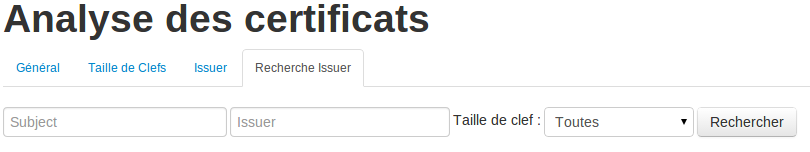
\includegraphics[scale=0.5]{images/site_web_search_bar.png}
\end{center}
\caption{Site Web - Bar de recherche}
\label{search_bar}
\end{figure}

La requête est envoyée sur le serveur via un appel en AJaX. Le résultat est alors affiché, avec un diagramme circulaire, pour représenter le nombre total de certificats et de certificats vulnérables contenus dans la base.

\begin{figure}[H]
\begin{center}
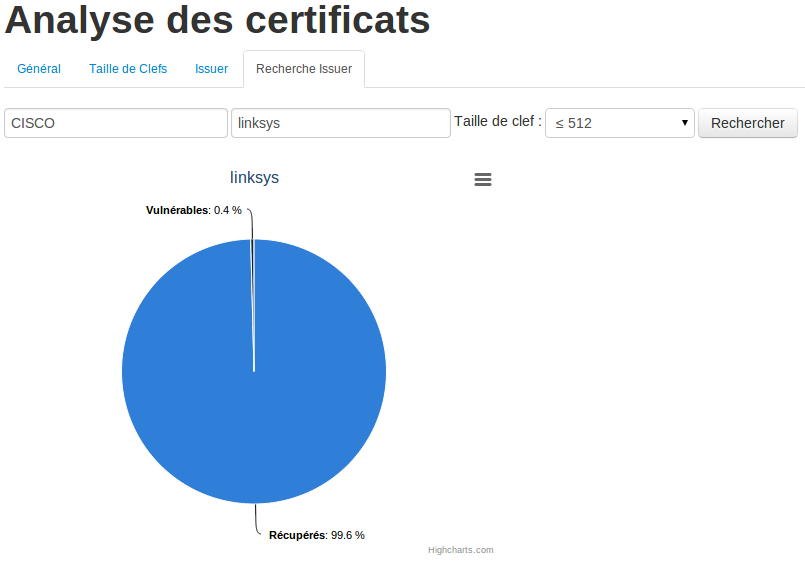
\includegraphics[scale=0.5]{images/site_web_search_result.png}
\end{center}
\caption{Site Web - Résultat d'une recherche}
\label{search_result}
\end{figure}

 
\section{Résumé d'audit}

Nous souhaitions, pour cette partie, intégrer le rapport d'audit directement sur le site web. De ce fait, nous avons utilisé un outil de conversion de fichier \textit{TeX} dans un dossier de fichiers \textit{HTML} que nous avons ensuite rejoins dans le dossier racine de notre site. Afin de garder la même mise en forme des pages web du site, nous avons modifié les différentes balises en y rajoutant les styles nécessaires.


\section{Test Navigateur Client}

Cette partie intègre l'outil permettant d'analyser les différentes \textit{ciphersuite} utilisées à l'établissement de connexion entre un client et un serveur, comme expliqué au chapitre \ref{analyseDynamique}. La page est divisé en 4 sections :
\begin{itemize}
\item Version et Algorithmes de chiffrements supportés ;
\item Algorithmes de signatures supportés ;
\item Courbes elliptiques ;
\item Légende.\\
\end{itemize}

\begin{figure}[H]
\begin{center}
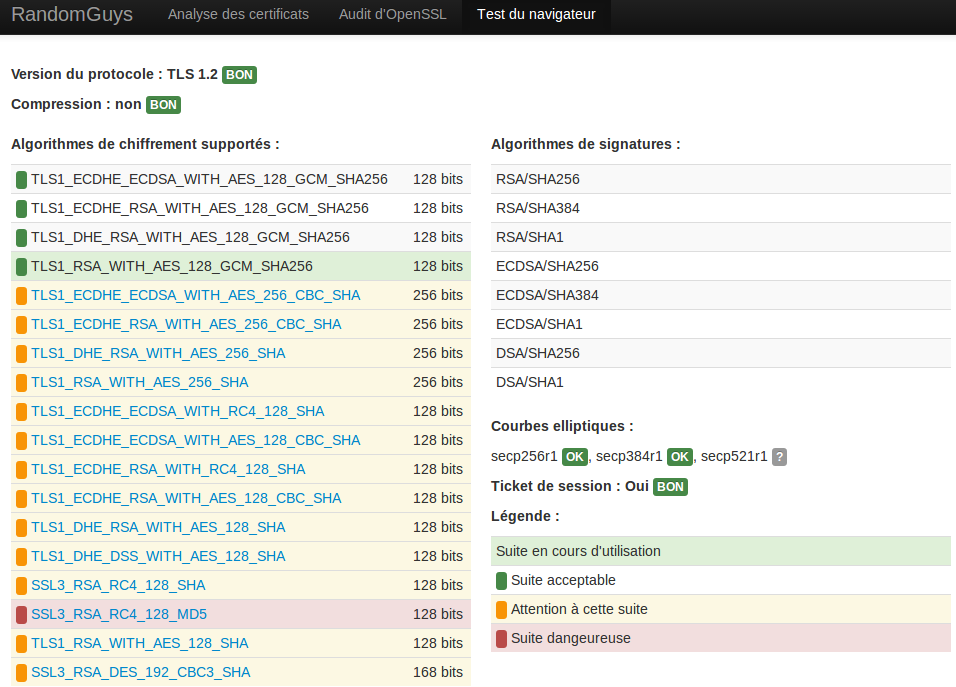
\includegraphics[scale=0.5]{images/site_web_test_client.png}
\end{center}
\caption{Site Web - Test du Navigateur}
\label{test_client}
\end{figure}